%==============================================================================
% BMEiCON 2026 — Stage 1 manuscript (IEEEtran conference format)
% Compile: pdflatex -> bibtex (none; refs are manual) -> pdflatex x2
% Requires: IEEEtran.cls (ships with most TeX distributions / CTAN)
%==============================================================================
\documentclass[conference]{IEEEtran}
\IEEEoverridecommandlockouts

\usepackage{cite}
\usepackage{amsmath,amssymb,amsfonts}
\usepackage{graphicx}
\graphicspath{{../../validation_outputs/}}
\usepackage{textcomp}
\usepackage{xcolor}
\usepackage{booktabs}
\usepackage{array}
\usepackage{url}
\usepackage{CJKutf8}   % for the 形似神不似 glyphs; remove if not needed
\usepackage[T1]{fontenc}

% Allow \shape... style inline code
\newcommand{\code}[1]{\texttt{#1}}

\begin{document}

\title{Spectrally Similar, Dynamically Invalid: A Single-Subject Diagnosis of
Loophole Exploitation in Neural Mass Model Fitting}

\author{\IEEEauthorblockN{Author Name(s)}
\IEEEauthorblockA{Affiliation\\
City, Country\\
email@domain}}

\maketitle

%------------------------------------------------------------------------------
\begin{abstract}
Personalized neural mass models for sleep EEG are commonly fitted with spectral
objectives. We show that such objectives can select solutions that are
spectrally similar to a target recording yet leave the intended sleep dynamics
unverified---and, when those dynamics are explicitly audited, invalid---a
failure we call \emph{shape-alike, spirit-unalike}
(\begin{CJK}{UTF8}{gbsn}形似神不似\end{CJK}). Using one Sleep-EDF subject
(SC4001, N3) and a neurolib thalamocortical model (ALN cortical node coupled to
a thalamic node), we diagnose this failure through an iterative V1--V7 fitting
history. A spectral-only baseline reached high residual spectral similarity
(\code{shape\_r}~$=0.8586$) but gave no event-level guarantees; auditing that
same solution against 12 event-level criteria shows it passes only 5/12,
failing sustained UP states (T3), SO sharpness and regularity (T4, T6), spindle
burstiness (T7), and the entire SO--spindle coupling triad (T9--T11, modulation
index $=0$). This makes ``spectrally similar yet dynamically invalid'' concrete
on a single solution rather than inferred from version history. Later versions
exposed further optimizer loopholes---persistent-DOWN solutions, SO--spindle
decoupling, fake spindle transients, unreachable spectral spindle rewards. V7
replaced those rewards with event-level constraints, raising feasible solutions
from 1/4960 (V6) to 364/4960 and yielding a point passing all 12 constraints.
Because reward targets, bounds, duration, and one spindle-width threshold
changed together, we report this trajectory as confounded and isolate the
threshold effect: only 156/4960 V7 points survive V6's stricter rule, so
roughly half the recovery is threshold relaxation. Two held-out checks give
mixed evidence: V7 is closer to real EEG on SO waveform morphology (RMSE $0.39$
vs $0.57$) but produces essentially zero cortical spindles, where V1 retains
some. We claim neither model is correct; the result is a single-subject
diagnostic existence claim and a transferable loophole-audit workflow.
\end{abstract}

\begin{IEEEkeywords}
sleep EEG, neural mass model, thalamocortical model, spectral fitting, slow
oscillation, sleep spindle, optimization, specification gaming
\end{IEEEkeywords}

%==============================================================================
\section{Introduction}
%==============================================================================
Personalized neural mass models are attractive tools for building mechanistic
``digital twins'' of brain rhythms. In sleep modeling, the target signals are
often summarized spectrally: N3 sleep is characterized by slow oscillations,
delta activity, and sleep spindles, and a fitted model is commonly judged by
whether its simulated power spectrum resembles the EEG target
\cite{cakan2023,jajcay2022,sleepedf}. Spectral matching is useful because it
compresses noisy electrophysiological time series into stable rhythm-level
summaries. However, it can also hide mechanistic errors. Two signals may share
similar spectral peaks while differing in whether they contain real UP/DOWN
alternation, waxing--waning spindle events, or coordinated slow-oscillation--
spindle coupling.

This paper diagnoses that failure mode in one subject: Sleep-EDF SC4001 during
N3 sleep. We call the failure \emph{shape-alike, spirit-unalike}
(\begin{CJK}{UTF8}{gbsn}形似神不似\end{CJK}): the simulated spectrum resembles
the target, but the underlying dynamics do not implement the intended sleep
physiology. The study is deliberately scoped as a single-subject diagnostic and
existence claim. It does not establish a population-level fitting method, nor
does it claim that the final model is globally more EEG-like on every metric.
Instead, it shows that a standard spectral objective can select a dynamically
invalid solution---one that fails an explicit event-level audit---and that the
iterative history of failed optimizers is itself evidence of objective
loopholes.

The key framing is to treat the optimizer as an adversarial loophole-searcher.
Differential evolution does not know the intended physiology; it only searches
for parameter settings that satisfy the objective it is given. If the objective
rewards spectral similarity without event-level safeguards, or if a constraint
admits a loophole, the optimizer can exploit it. Our V1--V7 development history
repeatedly exposed such failures: spectral-only fitting, weak dynamics
constraints, PAC-free spindle solutions, transient events masquerading as
spindles, and FOOOF-based rewards that were unreachable in the SO-stable
regime. V7 is the result of closing those specific loopholes with event-level
constraints and redesigned rewards.

In estimation terms, this is a statement about objective misspecification and
non-identifiability: a spectral summary does not uniquely determine the
underlying dynamics, so an objective built on it is satisfiable by dynamically
distinct solutions. Our contribution is not that observation, which is well
known, but its \emph{iterative operationalization}---treating differential
evolution as an adversary and using each feasibility collapse to localize a
specific objective loophole. The principle generalizes to any simulator fitted
to summary statistics; we keep the evidence single-subject by design.

The contributions are:
\begin{enumerate}
\item We demonstrate, in a single SC4001 N3 case study, that high spectral
similarity can coexist with dynamically invalid fitted solutions, and we make
this concrete by auditing the V1 spectral-only solution against the same
event-level criteria (Sec.~\ref{sec:resultsA}).
\item We present the V1--V7 fitting history as an empirical loophole audit of
the objective---an adversarial red-teaming protocol---rather than as an
implementation footnote.
\item We report both the positive event-level result and two independent
held-out checks that give mixed evidence (V7 closer on SO waveform morphology,
V1 closer on cortical spindle density), narrowing the claim to event-level
loophole closure rather than global superiority---and we surface a residual
loophole that survives inside the closed V7 audit.
\end{enumerate}

%==============================================================================
\section{Related Work}
%==============================================================================
\subsection{Neural mass fitting for sleep rhythms}
Neural mass and mean-field models have been used to reproduce macroscopic sleep
rhythms, including slow oscillations and spindle-band activity
\cite{cakan2023,jajcay2022,robinson2002}. These models provide mechanistic
structure beyond descriptive EEG statistics: parameters can represent cortical
excitability, adaptation, thalamic conductances, and thalamocortical coupling.
Prior work has often emphasized reproduction of rhythm-level or spectral
phenomena. Our work is complementary but more diagnostic: we ask whether
spectral matching is sufficient as an objective for personalization, and we
show that it can select solutions that satisfy spectral appearance while
failing event-level dynamics.

\subsection{Slow oscillation--spindle physiology}
N3 sleep is not defined by a spectrum alone. Slow oscillations involve
alternating DOWN and UP states in cortical activity \cite{steriade1993,
massimini2004}, while spindles appear as transient waxing--waning sigma-band
events associated with thalamocortical circuitry \cite{molle2011,helfrich2018}.
Coupling between slow-oscillation phase and spindle amplitude has been studied
as a marker of memory consolidation and sleep physiology
\cite{tort2010,canolty2006,mander2015}. These phenomena motivate event-level
constraints: a model should not merely have power in the correct bands; it
should produce plausible events with temporal structure. The event metrics used
here are deliberately aligned with established detection conventions rather than
invented: spindle event count and duration follow amplitude/duration criteria
in the spirit of standard detectors \cite{molle2011,ferrarelli2007} and open
implementations such as YASA \cite{vallat2021}, and the SO criteria follow
zero-crossing/amplitude conventions \cite{steriade1993,massimini2004}. The
thresholds attached to these metrics are empirical and subject-specific
(Sec.~\ref{sec:constraints}); the metric \emph{forms} are not.

\subsection{Optimizer loopholes and specification gaming}
The failure studied here resembles specification gaming in machine learning: an
optimizer exploits the literal objective rather than the designer's intended
goal \cite{krakovna2020,amodei2016}. In neural model fitting, a candidate can
score well by exploiting spectral artifacts, overly broad rewards, or
incomplete constraints. We import that adversarial-optimizer framing into
personalized sleep modeling. The claim is not that the optimizer is malicious,
but that objective functions define incentives; if the incentive misses
event-level physiology, the search can find shape-alike but dynamically invalid
solutions. Statically, this is the familiar problem of model/objective
misspecification and parameter non-identifiability. The framing earns its place
by converting a static property into a \emph{procedure}: each time a patched
objective is re-attacked and feasibility collapses, the collapse localizes the
next loophole. The reusable output is an audit workflow, not the
already-accepted conclusion that constraints help.

%==============================================================================
\section{Methods}
%==============================================================================
\subsection{Data and target spectrum}
We used Sleep-EDF subject SC4001 and selected N3 sleep epochs. EEG epochs are
aligned to the hypnogram, 30~s N3 epochs are extracted, epochs with
peak-to-peak amplitude above 200~$\mu$V are rejected, and Welch PSD estimates
are averaged across accepted epochs (channel \code{EEG Fpz-Cz}; 57 accepted N3
epochs enter the target PSD). The spectral fitting range is 0.5--20~Hz. The
held-out SO-waveform check (Sec.~\ref{sec:heldout}) uses a separate, larger
pool of 142 clean N3 epochs under its own QC and is independent of this target
PSD. We use ``slow oscillation'' (SO) for the $<\sim$1.25~Hz band that carries
the UP/DOWN alternation and ``delta'' for the $\sim$1--4~Hz band; the V7
selected point reports \code{T4\_freq}~$=1.25$~Hz, at this SO/delta boundary,
and is treated as SO here.

For the spectral similarity term, the target PSD is decomposed using
FOOOF/specparam-style aperiodic fitting \cite{donoghue2020}. The comparison is
not raw PSD correlation: both target and simulated PSDs are converted to
log-domain residual spectra after subtracting the fitted aperiodic background,
and \code{shape\_r} is the Pearson correlation between those residual spectra
after aligning the simulated PSD to the target FOOOF frequency grid. This makes
the objective more rhythm-specific than raw power matching, but the V1 result
shows that even this residual spectral objective does not guarantee correct
dynamics.

\subsection{Thalamocortical model and free parameters}
The simulator is a two-node thalamocortical mean-field model implemented with
neurolib's \code{MultiModel}: an ALN cortical node coupled to a thalamic node.
The fitting procedure searches over eight parameters: \code{mue}, \code{mui},
\code{b}, \code{tauA}, \code{g\_LK}, \code{g\_h}, \code{c\_th2ctx}, and
\code{c\_ctx2th}. These include cortical background inputs and adaptation
parameters, thalamic TCR conductances, and directed thalamocortical /
corticothalamic coupling strengths. Each candidate is simulated for 60~s at
1~kHz; the first 5~s are discarded as burn-in before any metric is computed.
The search uses \code{scipy.optimize.differential\_evolution}
(\code{strategy='best1bin'}, population size 20, 30 generations), and all
stochastic components (Ornstein--Uhlenbeck noise and node initialization) are
seeded deterministically (seed 42) so metrics are reproducible across calls
with identical parameters. Each reported version corresponds to a single DE run
under one seed; we therefore treat per-version feasible \emph{counts} as point
estimates without run-to-run variance and caution against over-reading small
differences (Sec.~\ref{sec:resultsB}).

\subsection{V7 fitness and feasibility}
The V7 feasible-solution reward is
\begin{equation}
\text{fitness} = 0.50\,\code{shape\_r} + 0.25\,\code{so\_power}
+ 0.25\,\code{spindle\_power},
\end{equation}
where \code{shape\_r} is the FOOOF residual spectral correlation above. Unlike
earlier versions, V7 computes \code{so\_power} and \code{spindle\_power} from
event-level quantities:
\begin{align}
\code{so\_power} &= \mathrm{clip}\!\left((\code{T4\_q}-1)/4,\,0,\,1\right),\\
\code{spindle\_power} &= \mathrm{clip}\!\left(\code{T12\_n\_verified}/15,\,0,\,1\right).
\end{align}
The denominators (4 and 15) are empirical reward-saturation scales, not
normative targets. In particular, 15 is the spindle-event count at which
\code{spindle\_power} saturates to 1 over the 60~s window; it is set above
realistic event counts to keep the reward discriminating among candidates, and
should be read purely as an internal normalization factor---not a claim that
physiological N3 contains 15 spindles per window (the held-out density measured
here is $\approx 2.4$--$3.0$ events/min, far lower;
Sec.~\ref{sec:heldout}).

This creates partial overlap between the reward and constraints, so we do not
treat the V7 fitness score as held-out validation. Instead the paper uses the
version history and feasibility audit as diagnostic evidence and separately
reports held-out checks. Infeasible points are ranked by continuous constraint
satisfaction rather than a single cliff penalty, preserving a search gradient:
candidates that nearly satisfy the audit are distinguished from those that fail
all checks, while all feasible solutions remain ranked above infeasible ones.

\subsection{Event-level constraints}\label{sec:constraints}
V7 uses 12 binary constraints in four physiological categories:
\begin{enumerate}
\item \textbf{Cortical bistability:} DOWN state, UP state, and sustained UP
duration (T1--T3).
\item \textbf{Slow-oscillation structure:} SO peak sharpness/frequency and
inter-burst-interval regularity (T4, T6).
\item \textbf{Spindle reality:} spindle spectral width, envelope burstiness,
event count/duration, and event-internal sigma verification (T5, T7, T8, T12).
\item \textbf{SO--spindle coordination:} PAC strength, phase preference, and
up/down-ratio / lag-like coupling metric (T9--T11).
\end{enumerate}
The metric forms are physiologically motivated, but the thresholds are
empirical and subject-specific; the paper does not claim every threshold is
literature-derived. Two points guard against the reading that constraints were
simply tuned until V7 passed. First, each constraint is motivated by a failure
observed in an \emph{earlier} version, independently of whether the final V7
point satisfies it: the UP-state tests (T1--T3) respond to persistent-DOWN
solutions in V2--V3; the PAC three-pack (T9--T11) responds to SO--spindle
decoupling in V5; and event-internal sigma verification (T12) responds to fake
spindle transients in V6. Each motivating diagnostic precedes the V7 reward
redesign and does not depend on its outcome. Second, the PAC metrics (T9--T11)
use a convention-free, cycle-by-cycle estimator rather than the
bandpass-plus-Hilbert phase used in early prototypes, which systematically
biased the preferred SO phase for spike-like firing-rate signals; we therefore
report PAC strength as a constraint but avoid preferred-phase point claims.

\subsection{Held-out checks}\label{sec:heldout}
To test whether event-level feasibility also improved independent statistics,
we implemented two held-out checks, neither of which calls the V7 constraint
function or reuses T1--T12, \code{shape\_r}, \code{so\_power}, or
\code{spindle\_power}.

\textbf{SO average-cycle morphology.} Real SC4001 N3 EEG and simulated cortical
activity are bandpassed to the SO range, aligned to SO cycle anchors,
normalized, averaged into templates, and compared by RMSE and correlation.

\textbf{Cortical spindle density.} Because the SO template primarily probes
low-frequency cycle shape and can look unremarkable even for degenerate event
dynamics, we add an event-level statistic disjoint from the audit: empirical
spindle density (events/min), measured with a standard sigma-band RMS detector
(band-pass to sigma, moving-RMS envelope, threshold $=$ mean $+$ 1.5$\cdot$SD,
accept events of 0.5--3.0~s). This detector is deliberately disjoint from the
fitness machinery: it operates on the \emph{cortical} (EEG-analog) signal,
whereas T8/T12 operate on the \emph{thalamic} signal; it uses a moving-RMS
envelope and mean$+$SD threshold, whereas T8 uses a 75th-percentile
Gaussian-smoothed Hilbert envelope and T12 adds Welch peak-inside verification;
and it uses 0.5--3.0~s duration bounds rather than T8's 0.3--2.0~s. We apply it
identically to real EEG and to the simulated cortical firing rate of V1 and V7,
over 300~s simulations and across two sigma bands (10--14~Hz, the model's
T-current resonance, and 11--15~Hz, the EEG sigma band), so the result is
robust to duration and band choice. Using a held-out statistic \emph{able} to
favor V7---not only one favoring V1---lets the event-level result be read in
either direction.

%==============================================================================
\section{Experiments}
%==============================================================================
\subsection{V1--V7 as an experimental design}
The evidence lies in the V1--V7 sequence, where each version exposed a new
objective loophole (Table~\ref{tab:loophole}).

\textbf{V1: spectral-only fitting.} The initial Fig.~7-style baseline used
FOOOF residual spectral similarity and SO/spindle spectral rewards. It reached
high spectral similarity (\code{shape\_r}~$=0.8586$) but imposed no event-level
guarantees---the cleanest exhibit for the claim that spectral fit can look good
without proving mechanistic validity.

\textbf{V2--V3: persistent-DOWN loophole.} Weak dynamics checks could be
satisfied by solutions with inadequate UP-state behavior. V3 added explicit
UP-state existence and sustained-UP tests, closing the persistent-DOWN
loophole.

\textbf{V4: constraints separated from rewards.} V4 separated feasibility
constraints from reward ranking and introduced SO sharpness, SO regularity, and
spindle envelope burstiness checks. It produced feasible solutions, but only
rarely (22/4703).

\textbf{V5: PAC constraints.} V5 added a three-part PAC audit to prevent
SO--spindle decoupling. The best solution still had \code{spindle\_power}~$=0$,
showing PAC constraints alone did not guarantee robust spindle rewards.

\textbf{V6: fake-spindle exposure.} V6 fixed T8 event detection and added T12 to
verify that detected events contain sigma-dominant oscillations. This made the
search stricter but exposed another failure: only 1/4960 evaluations were
feasible.

\textbf{V7: reward and bound redesign.} Diagnostics showed FOOOF spindle
rewards were effectively unreachable in SO-stable regimes, 30~s simulations made
T6 noisy, T5's original FWHM threshold rejected mechanistically valid narrow
spindles, and large \code{c\_th2ctx} destabilized cortical SO. V7 doubled
simulation duration to 60~s, replaced FOOOF SO/spindle rewards with
T4/T12-derived event rewards, tightened \code{c\_th2ctx}, and relaxed T5 FWHM to
admit narrow T-current resonance peaks.

\subsection{Evaluation measures}
We report: (1) best score and \code{shape\_r} for each version; (2) feasible
rate for versions with explicit feasibility rules; (3) V7 final T1--T12 metrics;
and (4) held-out SO waveform morphology distance and cortical spindle density.
The held-out results are not used to select V7; they test and constrain the
interpretation of V7's event-level improvements.

%==============================================================================
\section{Results}
%==============================================================================
\subsection{Spectral fit alone can look successful}\label{sec:resultsA}
The V1 spectral-only baseline achieved a high best \code{shape\_r}~$=0.8586$,
confirming the optimizer can find a solution whose FOOOF residual spectrum
resembles the target EEG. V1 did not enforce UP/DOWN alternation, spindle event
structure, event-internal sigma verification, or SO--spindle coupling.

To convert this from ``unchecked'' to ``demonstrably invalid,'' we evaluated the
canonical V1 selected parameter vector (the \code{shape\_r}~$=0.8586$ point)
through the \emph{same} event-level audit later formalized as V7's T1--T12,
using identical 60~s simulation, 5~s burn-in, and seed (42). The V1 point
passes only \textbf{5/12} constraints. It retains a DOWN state (T1) and a
momentary UP excursion (T2, max cortical rate 38.6~Hz), but fails: \textbf{T3}
---longest sustained UP state 86~ms, below the 100~ms threshold, so UP/DOWN
alternation is spiky rather than bistable; \textbf{T4}---SO spectral peak
$Q=1.68$ ($<2.0$), no sharp slow-oscillation peak; \textbf{T6}---inter-burst-
interval CV $=1.03$ ($\gg 0.4$), an irregular slow rhythm; \textbf{T7}---spindle-
envelope CV $=0.52$ ($<0.7$), not waxing--waning; and \textbf{T9--T11}---
modulation index exactly 0, a complete absence of SO--spindle coupling. The
corresponding cortical time series is shown in Fig.~\ref{fig:existence}. This is
the paper's existence object: a single solution spectrally similar to the target
(\code{shape\_r}~$=0.8586$) yet absent two core N3 phenomena---sustained UP
states and SO--spindle coupling. Re-scoring V1 under V7's audit adds no degrees
of freedom (the harness reproduces V7's stored 12/12 exactly, confirming
fidelity). Thus V1 is not merely unvalidated---under explicit audit it is
invalid on named criteria---while remaining spectrally convincing. For
reference, the V3 dynamics point also passes 5/12 (failing T4, T6, T7, T9--T11,
T12), so the spectral-versus-event gap is not unique to V1.

\subsection{Feasibility changed non-monotonically across versions}\label{sec:resultsB}
The feasible-rate trajectory (Table~\ref{tab:feasibility},
Fig.~\ref{fig:feasible}) supports the loophole-closure interpretation. The non-monotonic pattern matters: V5 and V6
did not simply improve over earlier versions; they became stricter and revealed
new failures. V7 recovered feasibility only after reward targets and bounds were
redesigned according to those diagnostics.

Two caveats keep this trajectory honest. First, the feasible \emph{rate} is not
a clean measure of loophole closure, because between V6 and V7 four things
changed at once: simulation duration (30 $\to$ 60~s, reducing T6 sampling
noise), the \code{c\_th2ctx} bound (tightened), the SO/spindle reward
definitions (FOOOF-based $\to$ reachable event-based), and the T5 spindle-width
threshold (relaxed from $>2.0$~Hz to $>0.2$~Hz, mechanically admitting narrow
T-current resonance peaks previously rejected). The last loosens a gate, so part
of the recovery is threshold relaxation rather than better physiology.
Re-scoring the V7 evaluation population under V6's original T5 threshold
isolates this: of V7's 364 feasible points, only 156/4960 remain feasible under
V6's strict $\code{FWHM}>2.0$~Hz rule, so 208 (57\%) of the recovery is
attributable to T5 relaxation alone and 156 to the duration/reward/bound
redesign. The V7 selected solution itself has spindle FWHM exactly 2.0~Hz: under
V6's strict threshold it would be infeasible, confirming T5 is load-bearing
rather than incidental. Second, because each version is a single seeded DE run,
small absolute counts are within plausible run-to-run variation; the V5-vs-V6
difference (5 vs 1) should not be read as meaningful, and we draw conclusions
only from the order-of-magnitude V6 $\to$ V7 shift after de-confounding.

\subsection{V7 selected point passed the event-level audit}
The selected V7 point passed all 12 constraints
(\code{n\_passed}~$=12$) with \code{score}~$=0.7759$, \code{shape\_r}~$=0.6226$,
\code{T4\_q}~$=4.433$, \code{T4\_freq}~$=1.25$~Hz, \code{T6\_ibi\_cv}~$=0.197$,
\code{T8\_n\_sp\_events}~$=25$, and \code{T12\_n\_verified}~$=20$.

This requires careful interpretation. V7's \code{shape\_r} is lower than V1's
spectral-only score, so V7 is not a better spectral fit. The comparison is also
not on identical ground: V1 searched broad bidirectional coupling bounds,
whereas V7 tightened \code{c\_th2ctx} for SO stability, so part of the
\code{shape\_r} gap reflects a smaller, more physiologically constrained search
space rather than a pure spectral/event trade-off. With that caveat, V7's
advantage is event-level feasibility: the final point satisfies the explicit
audit for cortical bistability, SO regularity, spindle event structure, and
SO--spindle coordination.

\subsection{Held-out checks give mixed evidence}\label{sec:resultsD}
We evaluated two held-out statistics, both on the canonical V1 point
(\code{shape\_r}~$=0.8586$).

\textbf{(1) SO average-cycle waveform morphology.} Using 142 clean SC4001 N3
epochs from \code{EEG Fpz-Cz}, the real template comprised 3881 SO snippets.
Distances to the real template are given in Table~\ref{tab:sowaveform}. On this
metric the canonical V1 point is the \emph{worst} of the three, and V7 is closer
to real EEG than V1 (RMSE $0.39$ vs $0.57$).

\textbf{(2) Cortical spindle density.} Real SC4001 N3 EEG has a cortical spindle
density of 2.41/min (10--14~Hz) to 2.96/min (11--15~Hz); the canonical V1 point
reaches 1.22--1.42/min---about half the real value---while V7 produces
\textbf{zero} cortical spindles in both bands over a 300~s simulation. On this
metric V1 is closer to real EEG than V7.

The two checks disagree: V7 is closer on SO morphology, V1 is closer on spindle
density. Neither is decisive. The SO average-cycle metric is narrow---it
normalizes amplitude and probes only low-frequency cycle shape---so V7's edge
there does not establish global fidelity; and V7's complete absence of cortical
spindles is a real deficiency the audit did not prevent
(Sec.~\ref{sec:residual}). We therefore retain only the audited-invalidity
claim (Sec.~\ref{sec:resultsA}) and disclaim any global ranking. This is why the
result settles on ``invalid'' (under explicit audit) rather than ``wrong'': the
audit demonstrates that the spectrally convincing V1 point violates named
event-level criteria, but the held-out evidence does not support the stronger
claim that either model is the more faithful one. V1 is not thereby
validated---it passes only 5/12 audit checks and under-produces cortical
spindles by about half---and V7, though it passes all 12, fails the cortical
spindle check. Neither solution is correct; the spectral objective and the event
audit each select a differently-deficient model.

%==============================================================================
\section{Discussion and Limitations}
%==============================================================================
\subsection{Main interpretation}
The central result is not that V7 is globally superior to V1. It is that V1
demonstrates the danger of spectral fitting: a high residual spectral score can
coexist with missing event-level guarantees. The V1--V7 sequence then shows how
the optimizer exploited each objective or constraint loophole until a more
explicit event-level audit was introduced. Under the adversarial-optimizer
framing, the post-hoc nature of several constraints is not something to hide---it
is evidence: each constraint was introduced because an apparently reasonable
previous objective admitted an unintended solution. The result is a diagnostic
methodology for discovering objective failures in personalized neural mass
fitting.

\subsection{Single-subject scope}
This is a single-subject case study. It demonstrates that the failure mode
exists for SC4001 N3, not that the same thresholds or final parameters
generalize across subjects. A population-level analysis would require repeating
the procedure across subjects and assessing whether the same loopholes and
constraint responses recur.

\subsection{Empirical thresholds}
The constraints combine physiologically interpretable metrics with empirical
thresholds. UP/DOWN states, spindle event duration, spindle envelope
burstiness, and PAC are grounded in sleep physiology, but the exact values used
here are subject- and model-specific. The manuscript should therefore be read as
a diagnostic study of objective failure, not as a universal definition of N3
physiology.

\subsection{Partial circularity}
V7's feasible-solution fitness includes a T4-derived SO reward and a
T12-derived spindle reward, creating overlap between fitness and constraints. We
therefore do not use the V7 score itself as held-out validation. Instead we
report the overlap explicitly and include two independent held-out checks
(Sec.~\ref{sec:resultsD}), which give mixed evidence and do not let us rank V1
against V7.

\subsection{Mixed held-out results}
The two held-out checks narrow the conclusion, and they disagree. On SO
average-cycle morphology, V7 is closer to real EEG than canonical V1 (RMSE
$0.39$ vs $0.57$); on cortical spindle density, V1 is closer because V7 produces
no cortical spindles at all. Together they prevent both the claim that V7 is
simply ``more EEG-like'' and the opposite claim that V1 is more EEG-like---the
held-out evidence does not rank the two. A model can pass the event audit while
still being deficient on an independent statistic (here, cortical spindle
expression), and a spectrally selected model can be closer on one waveform
statistic yet invalid under the audit. Neither model is correct: V1 fails 5/12
audit checks and under-produces cortical spindles, and V7, though it passes all
12, produces zero cortical spindles. The contribution is diagnostic, not a
ranking.

\subsection{Residual loophole: thalamic spindles without cortical expression}
\label{sec:residual}
The spindle-density check exposes a residual loophole inside the ``closed'' V7
audit, and it is the sharpest illustration of this paper's thesis. V7 passes T8
(25 detected spindle events) and T12 (20 sigma-verified events)---but those
constraints are evaluated on the \emph{thalamic} firing rate. Measured on the
\emph{cortical} signal, the EEG-analog quantity, V7 yields exactly \textbf{zero}
events over 300~s in both the 10--14~Hz and 11--15~Hz bands. The mechanism is
direct: V7's selected \code{c\_th2ctx}~$=0.0127$ is roughly eight times smaller
than V1's $0.099$, because V7 tightened thalamocortical coupling toward zero for
SO stability. At that coupling, thalamic spindles barely reach cortex, so the
events satisfying the audit would not appear in EEG.

This is specification gaming one level deeper than the failures V7 was designed
to close. The V7 audit verified spindle \emph{reality} (an event must contain a
genuine sigma oscillation, T12) but not spindle \emph{observability} in the
signal the EEG actually records. The optimizer, rewarded for thalamic spindle
events, found a regime that produces them on the unobserved node while the
SO-stability bound suppressed their cortical expression. The fix is
straightforward to state---verify spindles on the cortical signal, or constrain
\code{c\_th2ctx} from below---but the loophole was invisible until an
independent, signal-matched held-out check revealed it. It also reinforces that
V1 is no remedy: V1's larger coupling yields some cortical spindles
(1.2--1.4/min) but still only about half the real density (2.4--3.0/min), and V1
fails 5/12 audit checks. Both models are deficient in different ways; the audit
and the spectrum each hide a different failure.

\subsection{Stage 2 SBI}
Simulation-based inference is reserved for a future journal extension focused on
posterior identifiability. It addresses a different question---which parameters
are identifiable under selected summary statistics---and is not used here to
prove V7 superiority. This paper remains focused on Stage 1 objective diagnosis
and event-level loophole closure.

%==============================================================================
\section{Conclusion}
%==============================================================================
This single-subject diagnostic study shows that spectral objectives can select
thalamocortical model parameters that are shape-alike yet leave the intended
dynamics unverified---and that, when those dynamics are explicitly audited, the
spectrally convincing V1 solution is invalid on named event-level criteria (it
passes only 5 of 12 checks, with no sustained UP states and zero SO--spindle
coupling). Treating the optimizer as a loophole-searcher revealed a sequence of
failure modes across V1--V6, including persistent-DOWN behavior, SO--spindle
decoupling, fake spindle events, and unreachable spectral spindle rewards. V7
closed these event-level loopholes and increased feasible solutions from 1/4960
in V6 to 364/4960 (in part through threshold relaxation we quantify separately),
yielding a final point that passed all 12 event-level constraints. At the same
time, two independent held-out checks gave mixed evidence---V7 closer on SO
waveform morphology, V1 closer on cortical spindle density---and a residual
loophole emerged: V7 passes its thalamic spindle audit yet expresses zero
spindles in the EEG-analog cortical signal at its small thalamocortical
coupling. We therefore make no claim that V7 is the better model; V1 is itself
invalid under the audit (5/12) and under-produces cortical spindles by roughly
half. Both solutions are deficient in different ways. The contribution is not a
universal fitting method, nor a ranking of V1 against V7, but a transferable
diagnostic workflow: anchor a spectral objective, treat the optimizer as an
adversary, and use each feasibility collapse---and each independent held-out
check---to localize the next loophole, including loopholes that survive inside
an apparently closed audit. We report this for one subject; whether the same
loopholes recur across subjects is the natural next study.

%==============================================================================
% Tables
%==============================================================================
\begin{table}[!t]
\caption{Loophole-to-constraint map across V1--V7.}
\label{tab:loophole}
\centering
\footnotesize
\begin{tabular}{@{}p{0.55cm} p{3.2cm} p{3.3cm}@{}}
\toprule
Ver. & Loophole exposed & Constraint / change introduced \\
\midrule
V1 & Spectral fit without event guarantees & Baseline (FOOOF residual $+$ spectral SO/spindle rewards) \\
V2--V3 & Persistent-DOWN solutions & UP-state existence $+$ sustained-UP tests (T1--T3) \\
V4 & Rewards entangled with feasibility & Constraints separated; SO sharpness/regularity, spindle burstiness \\
V5 & SO--spindle decoupling & PAC three-pack (T9--T11) \\
V6 & Fake spindle transients & Event-internal sigma verification (T12) \\
V7 & Unreachable FOOOF rewards; noisy T6; over-strict T5; large \code{c\_th2ctx} & 60~s sims; T4/T12 event rewards; tightened \code{c\_th2ctx}; relaxed T5 \\
\bottomrule
\end{tabular}
\end{table}

\begin{table}[!t]
\caption{Version-level best score, \code{shape\_r}, and feasible rate. Under
V6's strict $\code{FWHM}>2.0$~Hz rule, only 156/4960 V7 points remain feasible
(208 of the 364 recovered, 57\%, are attributable to T5 relaxation).}
\label{tab:feasibility}
\centering
\footnotesize
\begin{tabular}{@{}l r r r@{}}
\toprule
Version & Best score & Best \code{shape\_r} & Feasible rate \\
\midrule
V1 & 0.8586 & 0.8586 & N/A \\
V3 & 0.7722 & 0.8334 & N/A \\
V4 & 0.4481 & 0.5449 & 22/4703 \\
V5 & 0.5296 & 0.5867 & 5/4960 \\
V6 & 0.3080 & 0.6159 & 1/4960 \\
V7 & 0.7759 & 0.6226 & 364/4960 \\
\bottomrule
\end{tabular}
\end{table}

\begin{table}[!t]
\caption{Held-out SO average-cycle waveform distances to the real SC4001
template (142 clean N3 epochs; 3881 SO snippets).}
\label{tab:sowaveform}
\centering
\footnotesize
\begin{tabular}{@{}l r r@{}}
\toprule
Version & RMSE & Correlation \\
\midrule
V1 canonical (\code{shape\_r}~$=0.8586$) & 0.5685 & 0.8390 \\
V3 dynamics & 0.3424 & 0.9414 \\
V7 event-constrained & 0.3909 & 0.9234 \\
\bottomrule
\end{tabular}
\end{table}

%==============================================================================
% Figures (placeholders; insert final artwork)
%==============================================================================
\begin{figure}[!t]
\centering
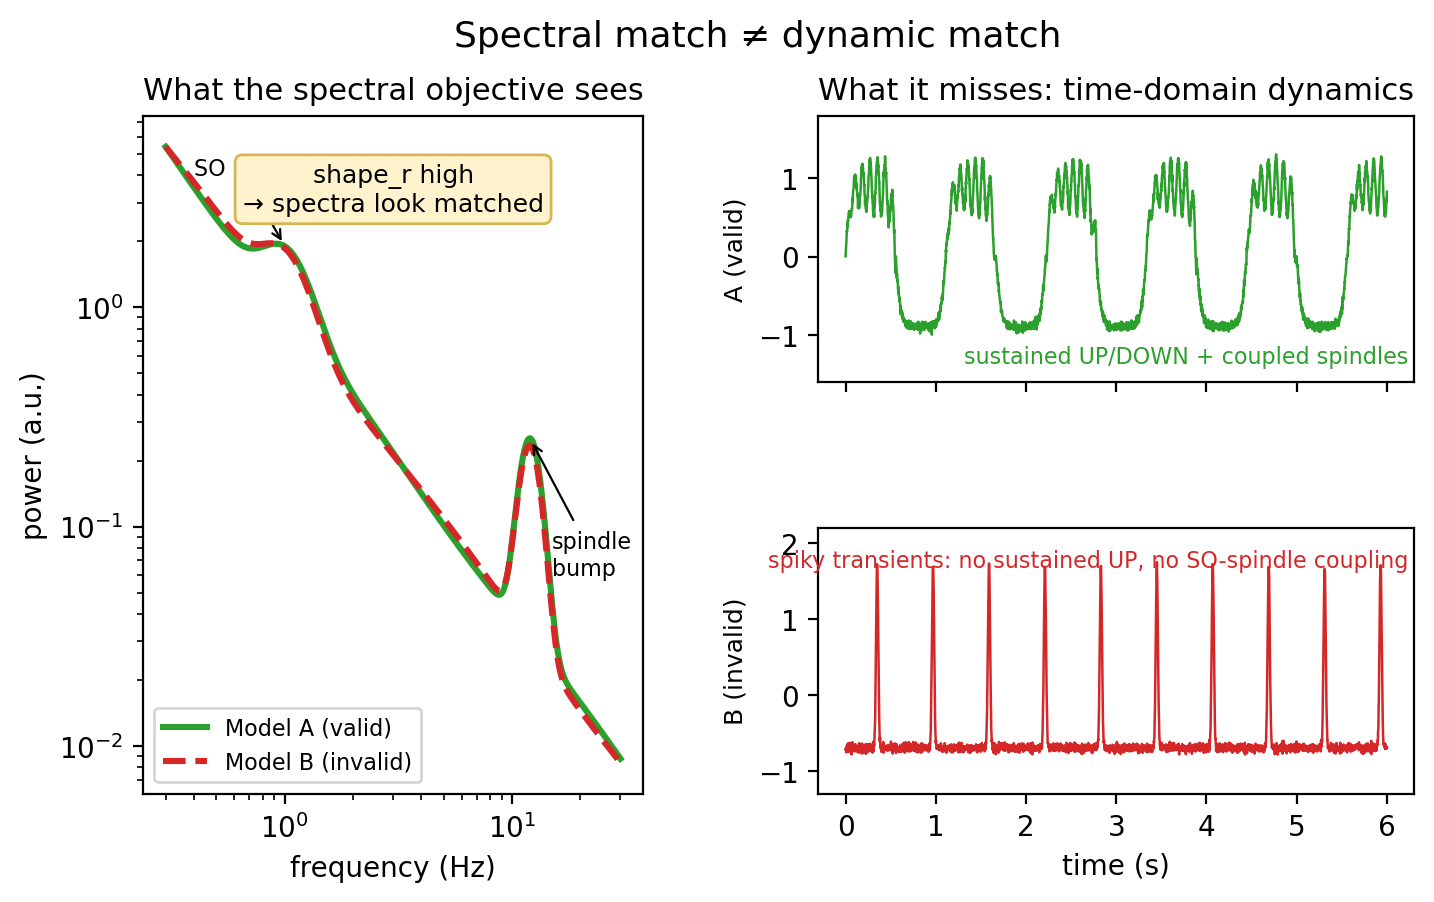
\includegraphics[width=\columnwidth]{fig_loophole_schematic.png}
\caption{Schematic of the spectral-fit loophole. Two models can share a nearly
identical power spectrum (left; high \code{shape\_r}) while differing sharply in
time-domain dynamics (right): Model~A shows sustained UP/DOWN bistability with
coupled spindles, whereas Model~B produces spiky transients with no sustained UP
state and no SO--spindle coupling. The spectral objective cannot separate them
(traces are illustrative).}
\label{fig:loophole}
\end{figure}

\begin{figure}[!t]
\centering
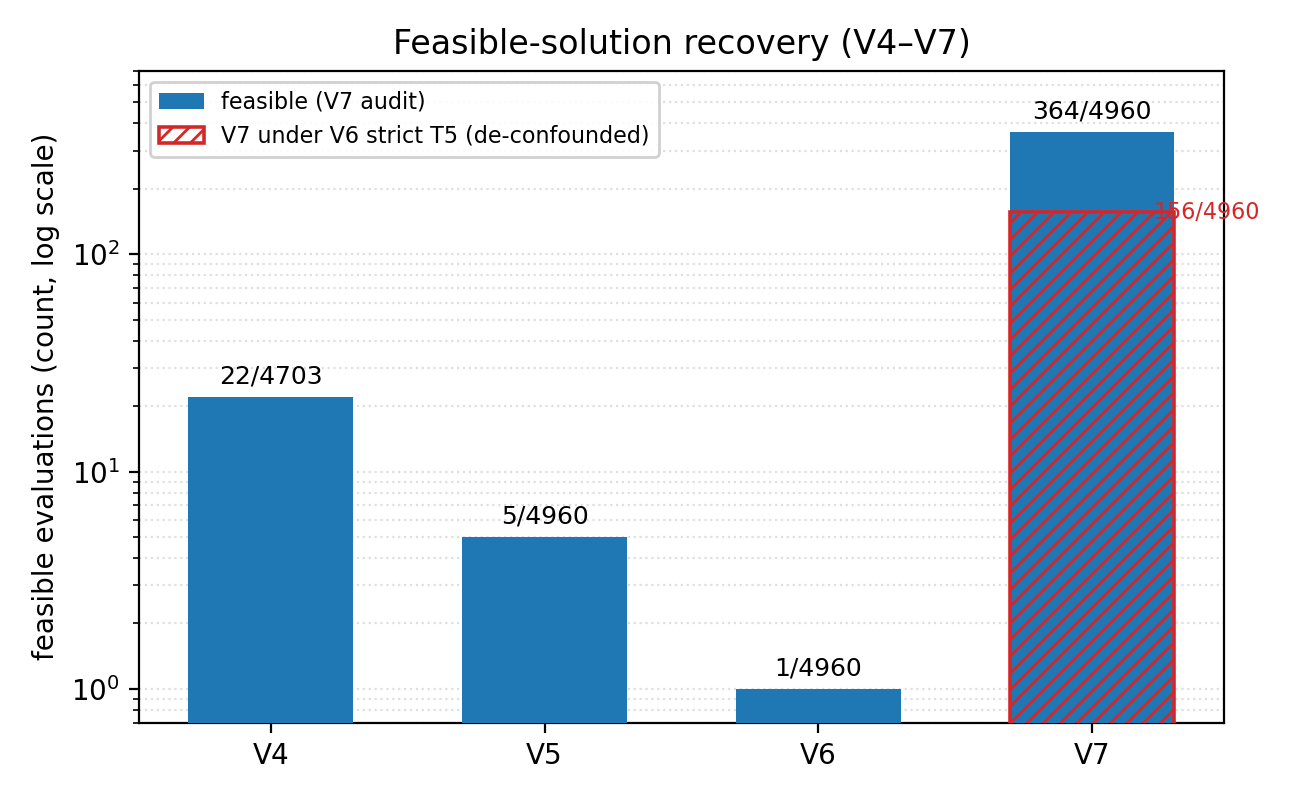
\includegraphics[width=\columnwidth]{fig_feasible_rate_recovery.png}
\caption{Feasible-solution recovery (V4--V7), log scale. Feasible counts fall
from 22/4703 (V4) to 1/4960 (V6) as constraints tighten, then jump to 364/4960
(V7) after the reward/bound redesign. The hatched overlay marks the 156/4960 V7
points that remain feasible under V6's strict $\code{FWHM}>2.0$~Hz rule---i.e.
$\approx$ half the recovery is T5 relaxation rather than loophole closure
(Sec.~\ref{sec:resultsB}).}
\label{fig:feasible}
\end{figure}

\begin{figure}[!t]
\centering
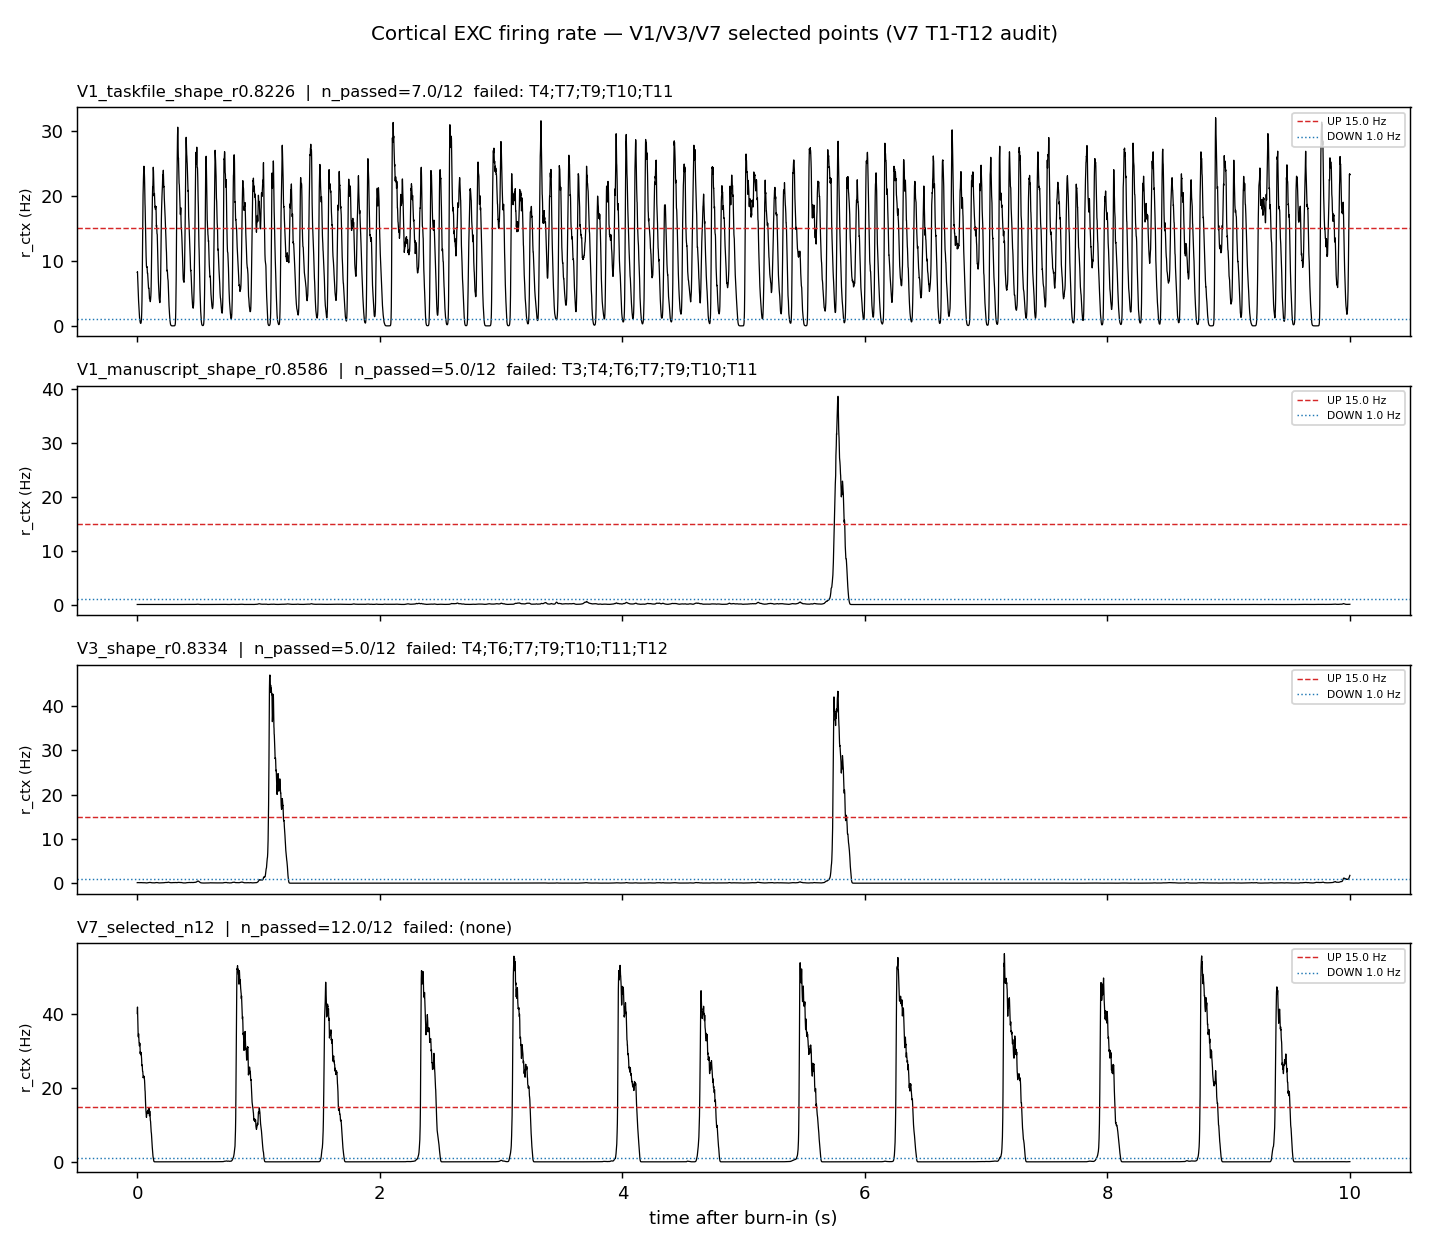
\includegraphics[width=\columnwidth]{fig_v1_v3_v7_t12_audit_timeseries.png}
\caption{Existence object---cortical excitatory firing rate of the V1, V3, and
V7 selected points under the same T1--T12 audit (60~s sim, 5~s burn-in,
seed~42). The canonical V1 point (\code{shape\_r}~$=0.8586$) passes only 5/12
and shows spiky UP excursions with no SO--spindle coupling, whereas V7 passes
12/12 with sustained UP/DOWN alternation; each panel annotates the failed checks
(Sec.~\ref{sec:resultsA}).}
\label{fig:existence}
\end{figure}

\begin{figure}[!t]
\centering
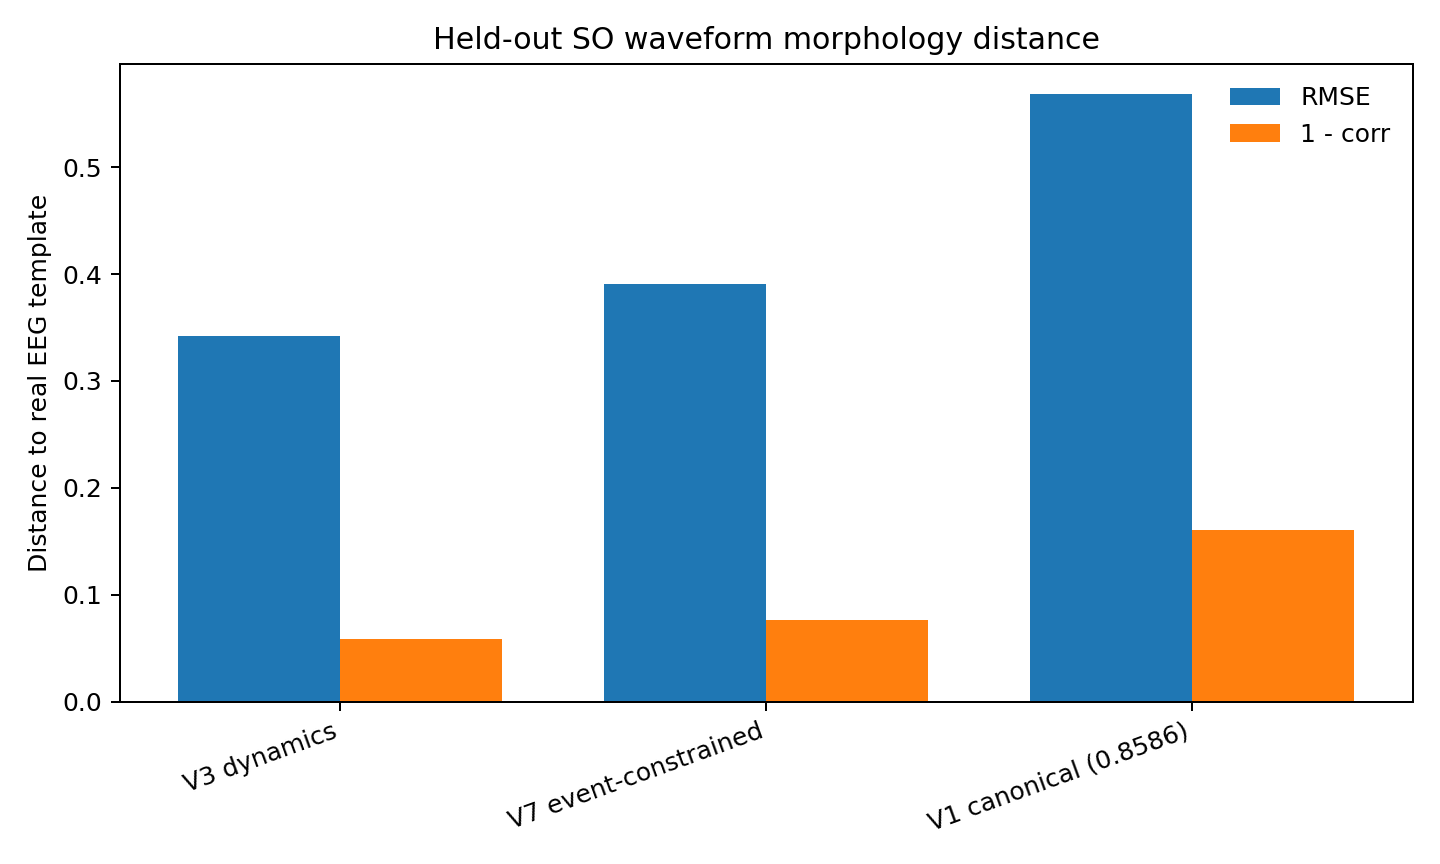
\includegraphics[width=\columnwidth]{fig_so_waveform_canonicalV1_distances.png}\\[2pt]
{\footnotesize (a)}\\[4pt]
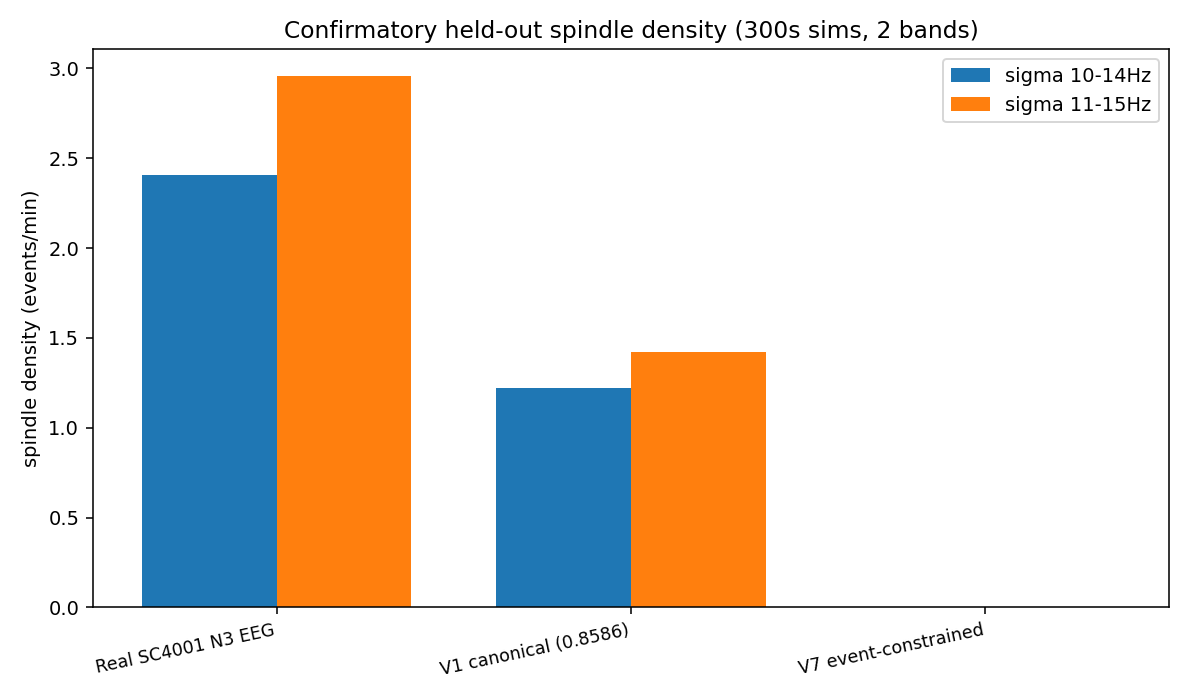
\includegraphics[width=\columnwidth]{fig_spindle_density_confirm.png}\\[2pt]
{\footnotesize (b)}
\caption{Held-out checks giving mixed evidence (canonical V1 throughout).
(a) SO average-cycle waveform distance to the real EEG template (RMSE and
$1-\mathrm{corr}$): V1 is the worst (RMSE 0.57), V7 (0.39) beats V1.
(b) Cortical spindle density over 300~s in two sigma bands: real EEG
$\approx 2.4$--$3.0$/min, V1 $\approx 1.2$--$1.4$/min, and V7 $=0$/min in both
10--14 and 11--15~Hz bands. The two checks disagree, so neither model is ranked
best overall.}
\label{fig:heldout}
\end{figure}

\begin{figure}[!t]
\centering
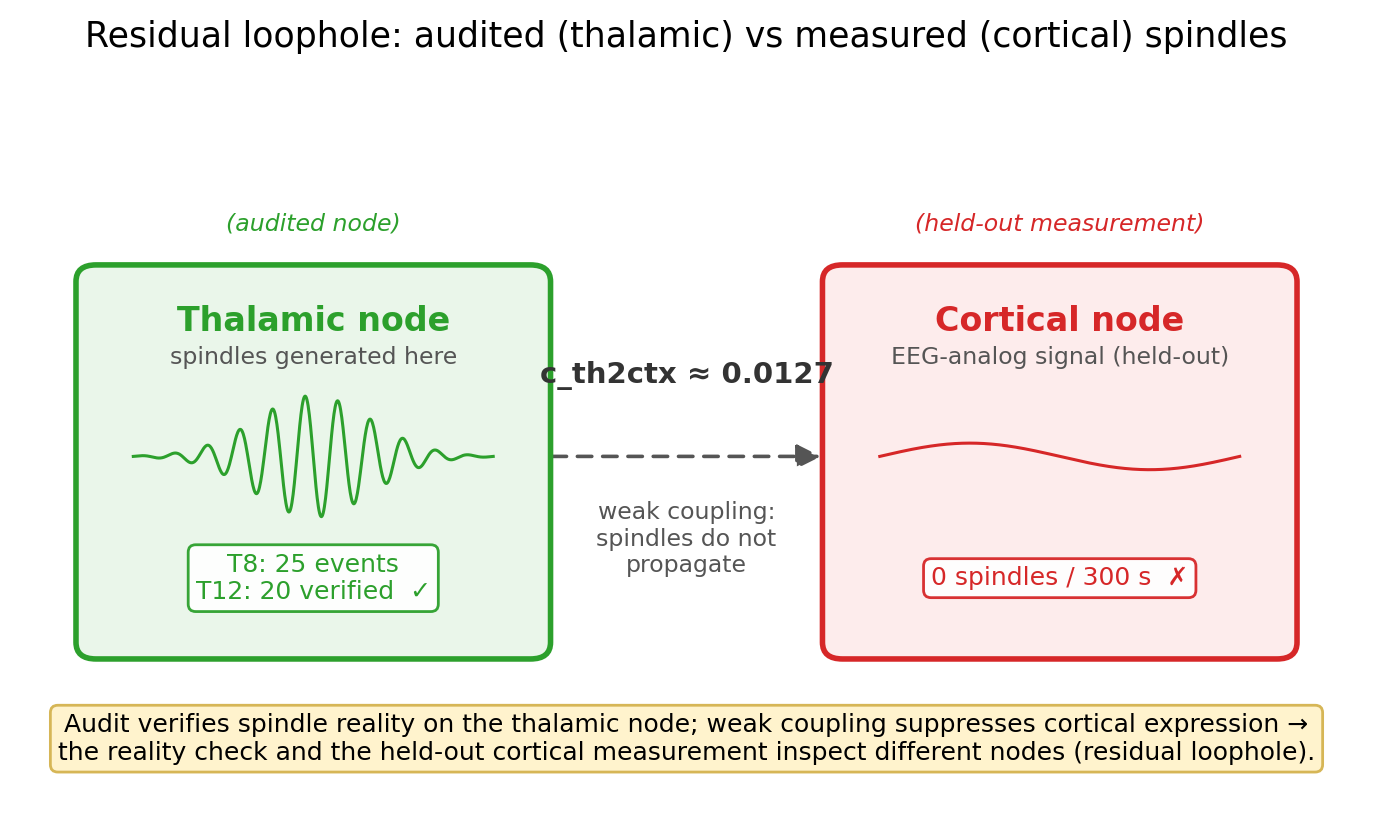
\includegraphics[width=\columnwidth]{fig_residual_loophole_schematic.png}
\caption{Residual-loophole schematic. V7's audit (T8/T12) verifies spindle
events on the thalamic node, but the EEG-analog signal is the cortical node. At
V7's small coupling (\code{c\_th2ctx}~$\approx 0.0127$) thalamic spindles do not
propagate, so cortical spindle density is $\approx 0$ even though the audit
passes---the reality check and the held-out measurement inspect different nodes.}
\label{fig:residual}
\end{figure}

%==============================================================================
% References
%==============================================================================
\begin{thebibliography}{99}

\bibitem{cakan2023} C. Cakan, N. Jajcay, and K. Obermayer, ``neurolib: A
Simulation Framework for Whole-Brain Neural Mass Modeling,'' \emph{Cognitive
Computation}, vol.~15, pp.~1132--1152, 2023, doi:10.1007/s12559-021-09931-9.

\bibitem{jajcay2022} N. Jajcay, C. Cakan, and K. Obermayer, ``Cross-Frequency
Slow Oscillation--Spindle Coupling in a Biophysically Realistic Thalamocortical
Neural Mass Model,'' \emph{Front. Comput. Neurosci.}, vol.~16, art.~769860,
2022, doi:10.3389/fncom.2022.769860.

\bibitem{sleepedf} B. Kemp, A. H. Zwinderman, B. Tuk, H. A. C. Kamphuisen, and
J. J. L. Oberye, ``Analysis of a sleep-dependent neuronal feedback loop: the
slow-wave microcontinuity of the EEG,'' \emph{IEEE Trans. Biomed. Eng.},
vol.~47, no.~9, pp.~1185--1194, 2000, doi:10.1109/10.867928. Database:
A. L. Goldberger \emph{et al.}, ``PhysioBank, PhysioToolkit, and PhysioNet,''
\emph{Circulation}, vol.~101, no.~23, pp.~e215--e220, 2000,
doi:10.1161/01.cir.101.23.e215.

\bibitem{robinson2002} P. A. Robinson, C. J. Rennie, and D. L. Rowe, ``Dynamics
of large-scale brain activity in normal arousal states and epileptic
seizures,'' \emph{Phys. Rev. E}, vol.~65, no.~4, art.~041924, 2002,
doi:10.1103/PhysRevE.65.041924.

\bibitem{steriade1993} M. Steriade, A. Nu\~nez, and F. Amzica, ``A novel slow
($<$1~Hz) oscillation of neocortical neurons in vivo: depolarizing and
hyperpolarizing components,'' \emph{J. Neurosci.}, vol.~13, no.~8,
pp.~3252--3265, 1993, doi:10.1523/JNEUROSCI.13-08-03252.1993.

\bibitem{massimini2004} M. Massimini, R. Huber, F. Ferrarelli, S. Hill, and
G. Tononi, ``The sleep slow oscillation as a traveling wave,'' \emph{J.
Neurosci.}, vol.~24, no.~31, pp.~6862--6870, 2004,
doi:10.1523/JNEUROSCI.1318-04.2004.

\bibitem{molle2011} M. M\"olle, T. O. Bergmann, L. Marshall, and J. Born,
``Fast and slow spindles during the sleep slow oscillation: disparate
coalescence and engagement in memory processing,'' \emph{Sleep}, vol.~34,
no.~10, pp.~1411--1421, 2011, doi:10.5665/SLEEP.1290.

\bibitem{helfrich2018} R. F. Helfrich, B. A. Mander, W. J. Jagust, R. T.
Knight, and M. P. Walker, ``Old brains come uncoupled in sleep: slow
wave--spindle synchrony, brain atrophy, and forgetting,'' \emph{Neuron},
vol.~97, no.~1, pp.~221--230.e4, 2018, doi:10.1016/j.neuron.2017.11.020.

\bibitem{tort2010} A. B. L. Tort, R. Komorowski, H. Eichenbaum, and N. Kopell,
``Measuring phase-amplitude coupling between neuronal oscillations of different
frequencies,'' \emph{J. Neurophysiol.}, vol.~104, no.~2, pp.~1195--1210, 2010,
doi:10.1152/jn.00106.2010.

\bibitem{canolty2006} R. T. Canolty \emph{et al.}, ``High gamma power is
phase-locked to theta oscillations in human neocortex,'' \emph{Science},
vol.~313, no.~5793, pp.~1626--1628, 2006, doi:10.1126/science.1128115.

\bibitem{mander2015} B. A. Mander \emph{et al.}, ``$\beta$-amyloid disrupts
human NREM slow waves and related hippocampus-dependent memory consolidation,''
\emph{Nat. Neurosci.}, vol.~18, no.~7, pp.~1051--1057, 2015,
doi:10.1038/nn.4035.

\bibitem{ferrarelli2007} F. Ferrarelli, R. Huber, M. J. Peterson, M. Massimini,
M. Murphy, B. A. Riedner, A. Watson, P. Bria, and G. Tononi, ``Reduced sleep
spindle activity in schizophrenia patients,'' \emph{Am. J. Psychiatry},
vol.~164, no.~3, pp.~483--492, 2007, doi:10.1176/ajp.2007.164.3.483.

\bibitem{vallat2021} R. Vallat and M. P. Walker, ``An open-source,
high-performance tool for automated sleep staging,'' \emph{eLife}, vol.~10,
art.~e70092, 2021, doi:10.7554/eLife.70092.

\bibitem{krakovna2020} V. Krakovna, J. Uesato, V. Mikulik, M. Rahtz,
T. Everitt, R. Kumar, Z. Kenton, J. Leike, and S. Legg, ``Specification gaming:
the flip side of AI ingenuity,'' DeepMind Safety Research, 2020.

\bibitem{amodei2016} D. Amodei, C. Olah, J. Steinhardt, P. Christiano,
J. Schulman, and D. Man\'e, ``Concrete Problems in AI Safety,''
arXiv:1606.06565, 2016; J. Skalse, N. H. R. Howe, D. Krasheninnikov, and
D. Krueger, ``Defining and Characterizing Reward Hacking,'' in \emph{Adv. Neural
Inf. Process. Syst. (NeurIPS)}, 2022, arXiv:2209.13085.

\bibitem{donoghue2020} T. Donoghue, M. Haller, E. J. Peterson, P. Varma,
P. Sebastian, R. Gao, T. Noto, A. H. Lara, J. D. Wallis, R. T. Knight,
A. Shestyuk, and B. Voytek, ``Parameterizing neural power spectra into periodic
and aperiodic components,'' \emph{Nat. Neurosci.}, vol.~23, pp.~1655--1665,
2020, doi:10.1038/s41593-020-00744-x.

\end{thebibliography}

\end{document}
